\documentclass{beamer}

\usepackage[utf8]{inputenc}
\usepackage[T1]{fontenc}
\usepackage{lmodern}
\usepackage{graphicx}
\usepackage{amsmath}
\usepackage[french]{babel}
\usepackage{array}

%\usetheme{Hannover}
\usetheme{Madrid}

\title[Analyse de iSudoku]{Analyse de iSudoku}
\subtitle[\ldots]{Projet de l'UE Ingénierie du Logiciel}
\author{
  Maude \bsc{Bellamy}
  \and
  Antoine \bsc{Houssais}
  \and
  Théo \bsc{Lebourg}
  \and
  Jérôme \bsc{Rahault}
  \and
  Fabricio \bsc{Santolin Da Silva}
  \and
  Simon \bsc{Tchernia}
}
\institute{Université Pierre et Marie Curie}
\date{\today}

\AtBeginSection[] {
  \begin{frame}
    \frametitle{Sommaire}
    \tableofcontents[currentsection, hideothersubsections, pausesubsections]
  \end{frame}
}

\begin{document}

\maketitle

\section{Présentation du groupe et de l’organisation}
\subsection{Gestion partagée des modèles et du code}
\begin{frame}
  \frametitle{Gestion partagée des modèles et du code}
  \begin{description}
    \item [Notre hébergeur de projet] \url{htps://github.com/neir/iSudoku}
      \pause
    \item [Notre logiciel de gestion de versions] Git
\end{description}
\end{frame}
\section{Phase d’analyse du iSudoku}
\subsection{Diagramme de cas d’utilisation}
\begin{frame}
\frametitle{Diagramme de cas d'utilisation}
\begin{figure}[h]
  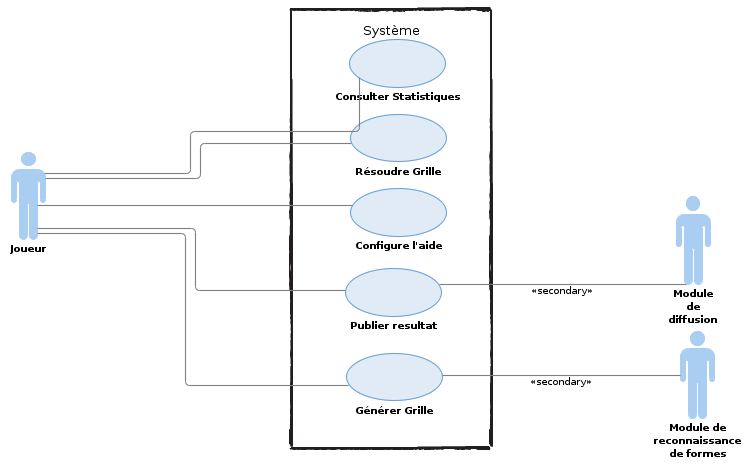
\includegraphics[scale=0.4]{diagrammeCasDUtilisation.png}
\end{figure}
\end{frame}
\subsection{Fiche détaillée de cas d’utilisations}
\begin{frame}
  \frametitle{Fiche détaillée du cas d'utilisation « Résoudre Grille »}
  \setbeamertemplate{blocks}[default]
  \begin{block}{\footnotesize{But}}
\scriptsize{L'utilisateur veut résoudre une nouvelle grille de sudoku}
  \end{block}
  \pause
  \begin{block}{\footnotesize{Séquencement}}
\scriptsize{Le cas d'utilisation commence lorsque la grille apparaît sur l'écran du
    smartphone / tablette}
  \end{block}
  \pause
  \begin{block}{\footnotesize{Enchaînement nominal}}
    \begin{enumerate}    
      \setbeamertemplate{enumerate item}[circle]
    \item
      \scriptsize{L'utilisateur sélectionne une case vide de la grille à remplir.}
    \item
      \scriptsize{Le système affiche une aide selon le niveau de difficulté :}
      \begin{itemize}
        \setbeamertemplate{itemize item}[circle]
      \item
        \scriptsize{facile : le système affiche pour chaque case les valeurs possibles au vu du
        reste de la grille}
      \item
        \scriptsize{difficile : le système n'affiche rien}
      \end{itemize}
    \item
      \scriptsize{L'utilisateur entre un numéro de 1 à 9 dans cette case.}
    \item
      \scriptsize{L'utilisateur répète l'action 1 jusqu'à compléter intégralement la grille.}
    \item
      \scriptsize{L'utilisateur valide la grille.}
    \end{enumerate}
  \end{block}
\end{frame}
\begin{frame}
\frametitle{Fiche détaillée du cas d'utilisation : « Résoudre Grille »}
\setbeamertemplate{blocks}[default]
  \begin{block}{\footnotesize{Post-conditions}}
    \scriptsize{Le QI du joueur est mis-à-jour}
  \end{block}
  \pause
  \begin{block}{\footnotesize{Enchaînement alternatif 1}}
    \scriptsize{Le niveau est intermédiaire et l’utilisateur se trompe lorsqu’il entre une valeur dans une case.
    L’enchaînement démarre après le point 3) de la séquence nominale :}
    \begin{enumerate}    
      \setbeamertemplate{enumerate item}[circle]
    \item
      \scriptsize{Le système affiche un message signalant que la valeur entrée est fausse}
    \item
      \scriptsize{On retourne au point 1 de la séquence nominale}
    \end{enumerate}
  \end{block}
  \pause
  \begin{block}{\footnotesize{Enchaînement alternatif 2}}
    \scriptsize{Le niveau est difficile et la grille remplie par l’utilisateur est fausse.
    L’enchaînement démarre après le point 5 de la séquence nominale :}
    \begin{enumerate}    
      \setbeamertemplate{enumerate item}[circle]
    \item
      \scriptsize{Le système affiche un message signalant que la grille est fausse et remet la grille à zéro.}
    \item
      \scriptsize{On retourne au point 1 de la séquence nominale}
    \end{enumerate}
  \end{block}
  \pause
  \begin{block}{\footnotesize{Enchaînement E 1}}
    \scriptsize{On interrompt le remplissage de la grille (ou bien l’utilisateur quitte, ou bien l’application est interrompue par une application externe comme la réception d’un appel).
L’enchaînement démarre après n’importe quel point de la séquence nominale.}
  \end{block}
\end{frame}
\begin{frame}
\frametitle{Diagramme de classe métier}
\begin{figure}[h]
  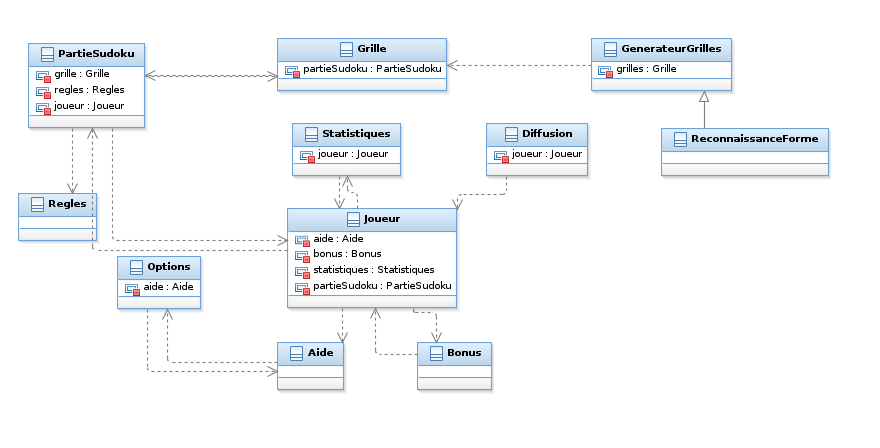
\includegraphics[scale=0.4]{diagrammeDeClasseMetier.png}
\end{figure}
\end{frame}
\end{document}
